\section{Recap: K-means}

\mode<presentation>{
\begin{frame} 
    \begin{center} \huge
        \secname
    \end{center}
	
\end{frame}
}

%%%%%%%%%%%%%%%%%%%%%%%%%%%%%%%%%%%%%%%%%%%%%%%%%%%%%%%%%%%%%%%
\begin{frame}{\secname: The setting}

\begin{itemize}
\item[] observations $\vec x \in \R^N$
\item[] $M$ clusters: $q_1, q_2, \ldots, q_M$
\item[] $M$ prototypes: $q_1, q_2, \ldots, q_M$
\item[] assignment variables for each point
\begin{equation}
\label{eq:assignment}
	m_q^{(\alpha)} := \left\{ \begin{array}{ll}
		1, & \text{if } \vec{x}^{(\alpha)} \text{ belongs to cluster } q
		\\\\
		0, & \text{otherwise}
	\end{array} \right. 
\end{equation}

\end{itemize}

\end{frame}

\begin{frame}{Inspecting a cluster}

\begin{center}
	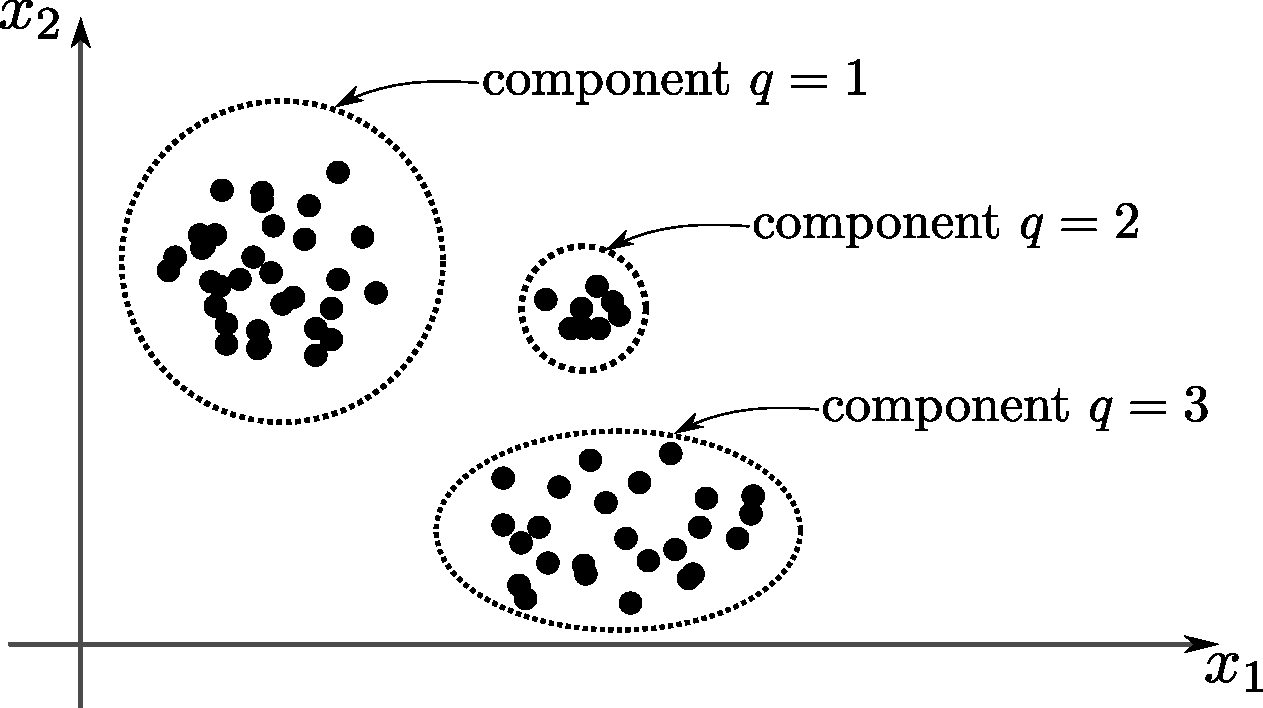
\includegraphics[width=0.5\textwidth]{img/fig1}
\end{center}

$\sum_{\alpha=1}^p m_q^{(\alpha)}$ counts how many points are assigned to cluster $q$ while $\frac{1}{p} \sum_{\alpha=1}^{p}
		\big( \vec{x}^{(\alpha)} - \vec{w}_q \big)^2$ yields the ``size''/variance of cluster $q$
		
\pause

\svspace{5mm}

The ``size'' does not tell us how \textit{important} a cluster is.

\end{frame}

\begin{frame}
\slidesonly{
\begin{center}
	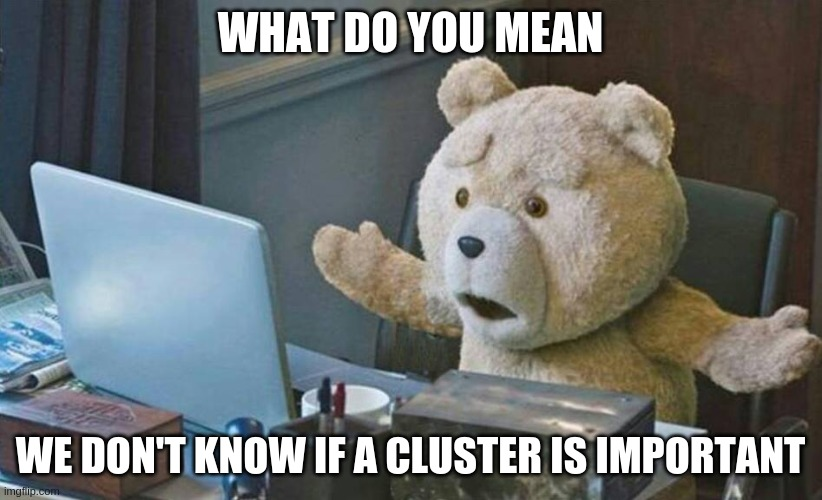
\includegraphics[width=0.5\textwidth]{img/meme_important}
\end{center}
}
\end{frame}

\begin{frame}{Importance of a cluster}

\only<1>{
\slidesonly{
\begin{center}
	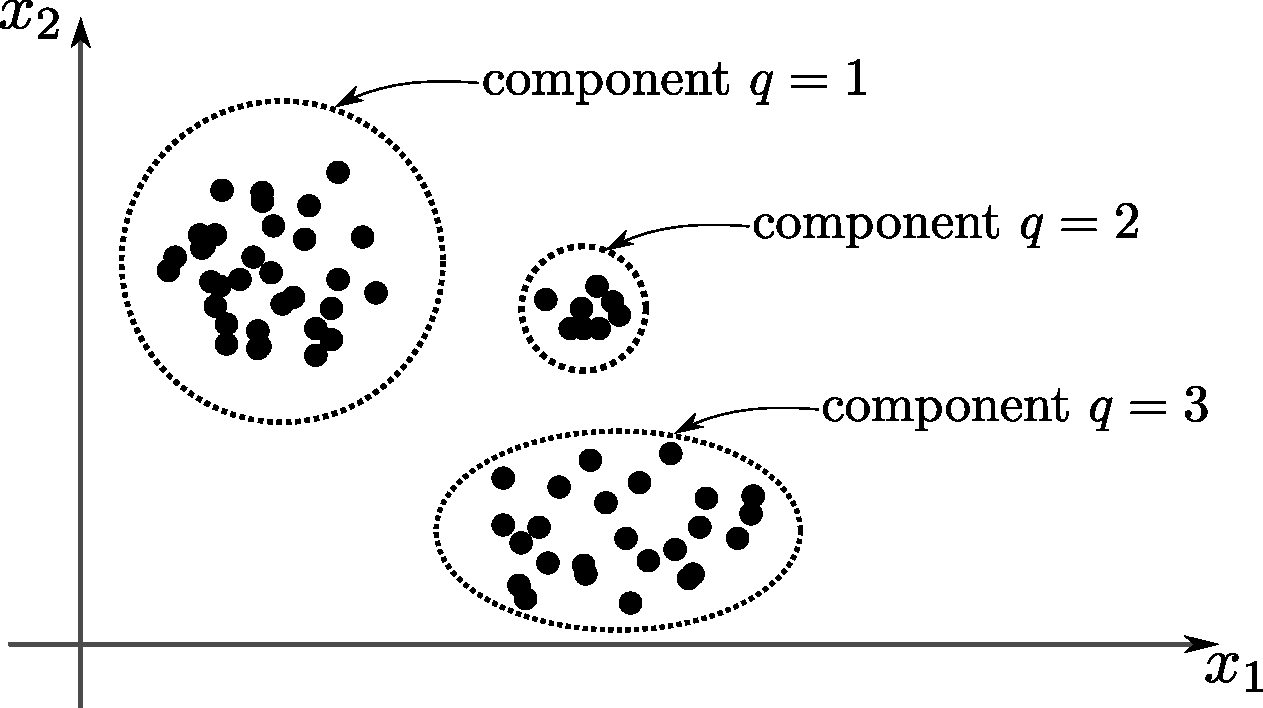
\includegraphics[width=0.5\textwidth]{img/fig1}
\end{center}
}
}

\only<1->{
Importance of a cluster:

\begin{center}
\hspace{12mm}high density \hspace{12mm}vs.\hspace{15mm}low density clusters\\
more $\longleftarrow$ importance $\longrightarrow$ less
\end{center}
Something that reflects how more or less data is generated in cluster $q_1$ vs. $q_2, q_3, \ldots$.
}

\only<2>{
\slidesonly{
\begin{center}
	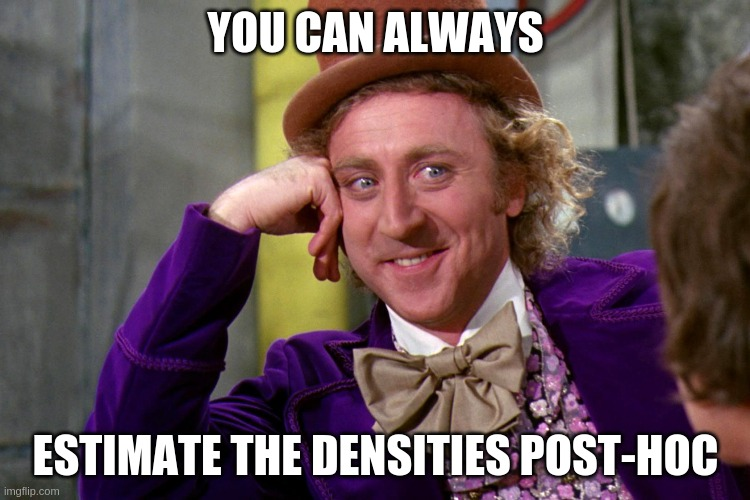
\includegraphics[width=0.3\textwidth]{img/meme_posthoc}
\end{center}
}
}
\only<3>{
\slidesonly{
\begin{center}
	
\includegraphics[width=0.4\textwidth]{img/meme_builtin}
\end{center}
}
}

\end{frame}

